\section{Preliminaries}
\label{sec:preliminaries}

We consider a digraph with non-negative real-valued edge weights and a finite set $V$ of $\abs{V}>1$ vertices represented by the adjacency matrix
\begin{align*}
  \MA := [a_{ij}]\in `R_+^{\abs{V}\times \abs{V}}.
\end{align*}
For convenience, we write
\begin{align*}
  w(B,C) := \sum_{i\in B}\sum_{j\in C} a_{ij} \quad \text{for }B,C\subseteq V,
\end{align*}
$w(i,C):=\sum_{j\in C}a_{ij}$ for $i\in V$, and similarly, $w(B,j):=\sum_{i\in B}a_{ij}$ for $j\in
V$. The weight $a_{ij}$ of edge $(i,j)\in V^2$ is taken to mean the influence of $i$ on $j$, which
needs not be equal to the influence $a_{ji}$ of $j$ on $i$ for $i\neq j$. In the following
definition, we generalizes the idea of web-communities in \cite{flake:efficient,
flake:cut-clustering} from graphs to digraphs.
\begin{definition}
  \label{def:support-community}
  A \emph{web community} is a non-empty subset $C\subseteq V$ of the vertices that satisfies
  \begin{align}
    \label{eq:support-community}
    w(i,C`/\Set{i}) > w(V`/ C,i), \ \forall i \in C,
  \end{align}
  i.e., the total external influence on each member of a web community is strictly smaller than the
  total influence the member has on other members of the community. 
\end{definition}
Note that singleton sets $\Set{i}$ for $i\in V$ are not web communities due to the strict inequality in \eqref{eq:support-community}. If $\MA$ is symmetric, which corresponds to a graph, the above definition reduces
to the original definition in \cite{flake:cut-clustering}. The following example shows that our extension is non-trivial as the web communities can depend on the directions of the edges.

\begin{example}
  \label{eg:directed-undirected}
  Consider the undirected graph in \figref{fig:eg-undirected} where $w(i,j)=1$ for $\Set{i,j}\in \Set{\Set{0,1},\Set{1,2}}$, and the digraph in \figref{fig:eg-directed} where $w(1,0)=2$ and $w(1,2)=w(2,1)=1$. The two graphs differ only in the directions of the edges, i.e., they have the same values of $w(i,j)+w(j,i)$ for all $i,j\in V$. However, the two graphs have different web communities: $\Set{0,1,2}$ for the undirected graph and $\Set{1,2}$ for the digraph. $\Set{0,1,2}$ is not a web community in the digraph in \figref{fig:eg-directed} since node~$0$ does not have any influence on other nodes, violating the condition~\eqref{eq:support-community}.
\end{example}

\begin{figure}
	\center
%	\def\figsep{-.19cm}
%	\def\dist{.9}
%	\def\disty{.9}
%	\def\s{.88}
	\def\figsep{.5cm}
	\def\dist{1}
	\def\disty{.9}
	\def\s{1}
	\subcaptionbox{\label{fig:eg-undirected}}{
		\begin{tikzpicture}[scale=\s, transform shape]
			\node(0) at (0,-1*\dist){$0$};
			\node(1) at (0*\dist,0){$1$};
			\node(2) at (1*\dist,0){$2$};
			%\node(2) at (1*\dist,-\dist){$2$};
			\draw (0)--node[left]{$1$}(1)--node[above]{$1$}(2);
		\end{tikzpicture}
	}
	\hspace{\figsep}
	\subcaptionbox{\label{fig:eg-directed}}{
		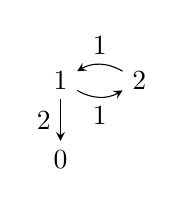
\begin{tikzpicture}[scale=\s, transform shape]
			\tikzset{edge/.style={<-, > = stealth}}
			\node(0) at (0,-1*\dist){$0$};
			\node(1) at (0*\dist,0){$1$};
			\node(2) at (1*\dist,0){$2$};
			\draw[edge] (0)--node[left]{$2$}(1);
			\draw[edge] (1) edge [bend left] node[above]{$1$}(2);
			\draw[edge] (2) edge [bend left] node[below]{$1$}(1);
		\end{tikzpicture}
	}
	\hspace{\figsep}
	\subcaptionbox{\label{fig:eg-disconnected}}{
		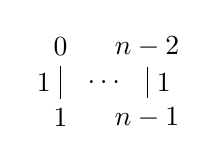
\begin{tikzpicture}[scale=\s, transform shape]
			\def\dist{.55}
			\tikzset{edge/.style={->, > = stealth}}
			\node(0) at (0,0){$0$};
			\node(1) at (0,-\disty){$1$};
			\node(dots) at (\dist,-\disty/2){$\dots$};
			\node(n-2) at (2*\dist,0){$n-2$};
			\node(n-1) at (2*\dist,-\disty){$n-1$};
			\draw(0)--node[left]{$1$} (1);
			\draw(n-2)--node[right]{$1$} (n-1);
		\end{tikzpicture}
	}\\
	\subcaptionbox{\label{fig:eg-chain}}{
		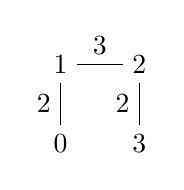
\begin{tikzpicture}[scale=\s, transform shape]
			\node(0) at (0*\dist,0){$0$};
			\node(1) at (0,1*\dist){$1$};
			\node(2) at (\dist,1*\dist){$2$};
			\node(3) at (\dist,0*\dist){$3$};
			\draw (0)--node[left]{$2$}(1)--node[above]{$3$}(2)--node[left]{$2$}(3);
		\end{tikzpicture}
	}
	\subcaptionbox{\label{fig:eg-dchain}}{
		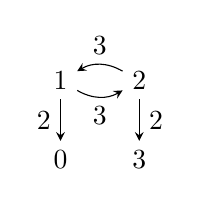
\begin{tikzpicture}[scale=\s, transform shape]
			\tikzset{edge/.style={<-, > = stealth}}
			\node(0) at (0*\dist,0){$0$};
			\node(1) at (0,1*\dist){$1$};
			\node(2) at (\dist,1*\dist){$2$};
			\node(3) at (\dist,0*\dist){$3$};
			\draw[edge] (0)--node[left]{$2$}(1); 
			\draw[edge] (3)--node[right]{$2$}(2); 
			\draw[edge] (1) edge[bend left] node[above]{$3$}(2);
			\draw[edge] (2) edge[bend left] node[below]{$3$}(1);
		\end{tikzpicture}
	}
	\subcaptionbox{\label{fig:eg-star}}{
		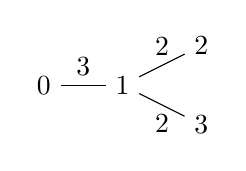
\begin{tikzpicture}[scale=\s, transform shape]
			\node(0) at (0,0){$0$};
			\node(1) at (1*\dist,0){$1$};
			\node(2) at (2*\dist,.5*\dist){$2$};
			\node(3) at (2*\dist,-.5*\dist){$3$};
			\draw (1)edge node[above]{$3$}(0) edge node[above]{$2$}(2) edge node[below]{$2$}(3);
		\end{tikzpicture}
	}
	%\caption{The weighted graphs for Examples~\ref{eg:directed-undirected} and \ref{eg:too-many-communities}}
	\caption{The weighted graphs for Examples~\ref{eg:directed-undirected}--\ref{eg:chain-cut}}
        \label{fig:eg12}
\end{figure}

An issue with the above definition of communities is that there can be exponentially many of them as illustrated below.

\begin{example}
  \label{eg:too-many-communities}
  For the graph in \figref{fig:eg-disconnected} where the edges with non-negative weights form a perfect matching, the web communities are all the non-empty subsets of the matched pairs. The number of communities is $2^{\abs{V}/2}-1$, which is exponential in $\abs{V}$.
\end{example}

Since there can be exponentially many web communities, it is impractical to enumerate all of them for a large graph. Even for graphs of moderate sizes, returning many communities without any form of organization or measures of qualities are not helpful, especially if the goal is to study a large graphical network by breaking it down into subnetworks. 

In the case when the graph is undirected, \cite{flake:cut-clustering} proposed the cut-clustering algorithm below: 
\begin{enumerate}
\item For any parameter $`a\in `R$, add a new node $s$ to the graph.
\item For each node $t\in V$, add an edge between $s$ and $t$ with weight $`a$.
\item Construct a Gomory-Hu tree of the graph. Remove $s$ and return the resulting connected components, which is a partition of $V$. If the Gomory-Hu tree is not unique, construct the tree that gives the finest partition.
\end{enumerate}
The above procedure is called cut-clustering, as each connected component returned corresponds to an $s$--$t$ mincut of the original graph augmented with the node $s$, by the property of the Gomory-Hu tree. We will call the non-singleton components as cut-clusters at threshold $`a$. It was shown that $`a$ serves as a parameter that measures the quality of the returned clusters in terms of graph expansion~\cite[(3.3)]{flake:cut-clustering}. However, the extension to digraphs is unclear since Gomory-Hu tree is defined for undirected graphs. There is also a limitation that the returned cut-clusters may not be web communities as one of the nodes in a cut cluster can fail to satisfy \eqref{eq:support-community}~\cite[Lemma~3.1]{flake:cut-clustering}.